\documentclass{SBCbookchapter}
\usepackage[utf8]{inputenc}
\usepackage[T1]{fontenc}
\usepackage[english,brazilian]{babel}
\usepackage{graphicx}
\usepackage{color} % colorir texto
\usepackage[colorinlistoftodos,prependcaption,textsize=tiny]{todonotes}

\newcommand{\rg}[1]{\todo[linecolor=blue,backgroundcolor=blue!25]{RG: #1}}

\title{Desenvolvimento de aplicações multimídia usando GStreamer}
\author{XXX, YYY, ZZZ}

\begin{document}
\maketitle
\begin{abstract}
\begin{otherlanguage}{english}
\end{otherlanguage}
\end{abstract}

\begin{resumo}
Este minicurso tem como objetivo apresentar os conceitos básicos de programação
de aplicações multimídia utilizando o Gstreamer.  GStreamer é um poderoso e
flexível framework multimídia, disponível em código livre, baseado no conceito
de~\emph{dataflow} e que permite o desenvolvimento de aplicações multimídia
avançadas---e.g., aquelas que requerem o sincronismo fino entre os diversos
objetos de mídia que fazem parte da apresentação.  Após apresentar os conceitos
básicos do GStreamer, o minicurso avança, em uma abordagem prática, discutindo
exemplos básicos de como aplicar/criar novos filtros e como estender o
\emph{framework} por meio de \emph{plugins}.  Ao final do minicurso é esperado
que os participantes tenham uma visão geraldo modelo de programação multimídia
baseado em \emph{dataflow} e do framework GStreamer, que estejam aptos a criar
aplicações básicas sincronizando áudio e vídeo, e que tenham a base para que
possam desenvolver seus próprios projetos~(mais avançados) no futuro.
\end{resumo}


\section{Justificativa de interesse e atração do público alvo}
Este minicurso tem como objetivo apresentar os conceitos básicos de programação
baseado em dataflow multimídia usando o GStreamer.
GStreamer~\cite{?} é um \emph{framework} multimídia disponível em código livre,
escrito em C (e com \emph{bindings} para várias outras linguagens), que usa a
abstração de \emph{dataflow}~\cite{?}. Atualmente, é um dos \emph{frameworks}
mais utilizados para o desenvolvimento de aplicações multimídia, sendo
o \emph{backend} em softwares como Totem~\cite{?}, AmaroK~\cite{?},
Rhythmbox~\cite{?}, GNOME Videos~\cite{?}, entre outros.

O \emph{framework} pode ser dividido em três partes: \emph{core},
\emph{plugins} e ferramentas. O \emph{core} implementa a arquitetura base que
suporta o fluxo de dados em um pipeline composto por diversos \emph{plugins}. 
\emph{Plugins} são interligados entre si e processam o conteúdo multimídia
(i.e., de/codificação, de/multiplexação, filtros, renderização, etc).
Finalmente, diversas ferramentas estão disponíveis para facilitar
o uso do \emph{framework}. Exemplos de ferramentas são o 
\emph{gst-inspector} (lista os plugins instalados) e o \emph{gst-launch}
(utilizado para construir pipelines simples via linha de comando).

Desenvolver aplicações usando o GStreamer pode ser descrito como a
especificação dos componentes que fazem parte de um \emph{pipeline}
(vide~Figura~\ref{fig:pipeline}), por onde os dados fluem a partir de uma fonte
de dados, são processados por diversos componentes intermediários até
finalmente serem renderizados, salvos em disco ou enviados pela rede.

\begin{figure}[ht!]
  \label{fig:pipeline}
  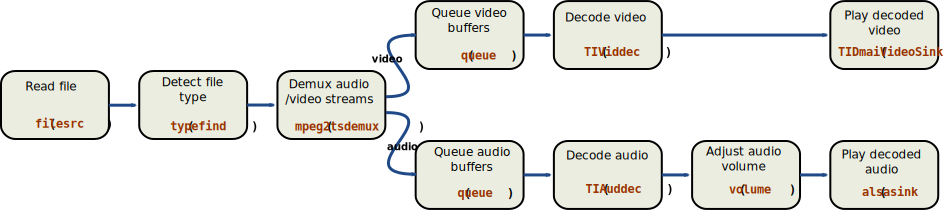
\includegraphics[width=\textwidth]{gstreamer_pipeline.pdf}
  \caption{Exemplo de um pipeline multimídia criado com o gstreamer.}
\end{figure}

Ao apresentarmos a base conceitual do modelo de programação baseado em
\emph{dataflow} e a abordagem prática usando o GStreamer, esperamos que este
minicurso possa criar a base, teórica e prática, para que os participantes
possam, no futuro, desenvolver suas próprias aplicações multimídia.  Em
especial, o modelo de programação em \emph{dataflow} pode ser útil em vários
cenários de aplicações multimídia, tais como editores de vídeo, transcorders,
transmissores de streaming de mídia, players de mídia e players de linguagens
multimídia.  Dessa forma, acreditamos que boa parte do público do WebMedia---em
especial aqueles interessados no desenvolvimento de aplicações e sistemas
multimídia---podem tirar proveito deste minicurso e dos conceitos que serão
apresentados.

Nativamente, o GStreamer já suporta uma grande variedade de componentes para
lidar com diferentes tipos de mídias, tais como componentes para a reprodução
de áudio, reprodução de áudio e video (sincronizados), gravação,
\emph{streaming} e edição.  Esses componentes podem ser integrados de várias
formas pelo programador para criar o pipeline multimídia de uma aplicação,
permitindo assim grande flexibilidade e podendo ser aplicados a diferentes
cenários de aplicações multimídia. Nesse sentido, aqueles interessados em
desenvolver aplicações multimídia para usuários finais podem tirar proveito
deste minicurso. 

Mais ainda, o GStreamer possui uma arquitetura modularizada, facilmente
extensível por \emph{plugins}. Para aqueles trabalhando com codificação,
processamento e renderização de monomídias, o desenvolvimento de plugins para
o GStreamer~(conteúdo também abordado no minicurso) pode ser útil para que
outros possam utilizar o seu trabalho em diferentes contextos.

Finalmente, aqueles que trabalham sistemas e linguagens multimídias~(e.g., NCL,
SMIL, HTML, etc.) também podem tirar proveito do minicurso. Em especial, o
modelo de dataflow e o GStreamer podem ser utilizados como base para o
desenvolvimento de middlewares de linguagens multimídia com o objetivo de
garantir o sincronismo fino entre as diversas mídias que fazem parte da
apresentação multimídia. Outra possível apliação é o desenvolvimento de APIs de
mais alto nível que também podem utilizar o GStreamer como \emph{backend}.

Além disso, outra motivação para este minicurso é que embora seja utilizado
como base para várias aplicações multimídia atualmente, a documentação
disponível em português sobre o GStreamer ainda é escassa. Dessa forma, este
minicurso também tem o potencial de servir como referência sobre o GStreamer
para a comunidade brasileira de multimídia.

%Além disso, a maior parte dessa documentação está em Inglês.
%[Colocar mais coisa aqui, e.g., disponibilidade, flexibilidade, controle
%  fino, base para aplicações mais complexas, etc.]

\section{Público-alvo}
O público-alvo principal deste minicurso são programadores, alunos de graduação
e de pós-graduação interessados em desenvolver aplicações multimídia
e sistemas multimídia~\cite{?}.  Os alunos devem possuir conhecimento básico da
linguagem~C~\cite{?} e estarem familiarizados com algum ambiente de
desenvolvimento para essa linguagem.  Como o minicurso será ministrado em um
ambiente Linux, é desejável que o público tenha conhecimento básico de alguma
distribuição.


\section{Sumário}
O minicurso está planejado para ser ministrado em oito módulos, são eles:

\begin{enumerate}
\item\emph{Introdução ao GStreamer}.  Apresentação do \emph{framework}
  multimídia GStreamer: histórico, arquitetura básica, licença, quem usa,
  dependências, formatos e plataformas suportadas.  E discutimos brevemente
  o seu modelo de programação, viz., \emph{dataflow} (ou \emph{pipeline})
  multimídia~\cite{?}.

\item\emph{Olá mundo: Tocando um vídeo}.  Apresentação de uma aplicação
  GStreamer básica que toca um vídeo e termina.  Esse exemplo utiliza a API
  de alto-nível~\texttt{GstPlayer}---atualmente a forma mais simples de se
  reproduzir um áudio ou vídeo no GStreamer.

\item\emph{Conceitos básicos: Destrinchando o exemplo anterior}.  Discutimos
  o que está por trás do código aparentemente simples do exemplo anterior.
  Começamos mostrando o \emph{pipeline} que a API~\texttt{GstPlayer} usa
  para reproduzir o vídeo e aproveitamos esse exemplo para introduzir cada
  um dos conceitos básicos do \emph{framework}:  \emph{element}, \emph{pad},
  \emph{caps}, \emph{clock}, \emph{buffer}, \emph{event}, \emph{message},
  \emph{bus}, \emph{bin} e \emph{pipeline}.  Após discutir os conceitos,
  voltamos à pratica e reimplementamos o exemplo do tópico anterior usando a
  API básica do GStreamer.  (Apesar da API~\texttt{GstPlayer} simplificar a
  programação de reprodutores de mídia, ela é inflexível e limita os
  possíveis usos do framework.  Dessa forma, é importante que os alunos do
  minicurso conheçam a API básica do GStreamer e seu modo de operação.)
  Ainda neste tópico, discutimos as ferramentas~\texttt{gst-inspect}, que
  consulta os elementos instalados no sistema, e ~\texttt{gst-launch}, que
  constrói um \emph{pipeline} na linha de comando.

\item\emph{Entrada e saída}.%
  \rg{O que vocês acham de colocarmos isso para o final? Depois de plugins?}
  Adicionamos suporte à entrada do usuário
  (teclado e mouse) ao exemplo anterior, e discutimos como os
  elementos~\texttt{appsrc} e~\texttt{appsink} podem ser utilizados para
  injetar ou obter dados do \emph{pipeline}.  Concluímos o tópico mostrando
  como renderizar os quadros produzidos no exemplo numa
  janela~GTK+~\cite{?}.

\item\emph{Filtros}.  Apresentamos os principais filtros de aúdio e vídeo
  disponíveis no GStreamer e discutimos como integrá-los ao exemplo.  Nesse
  ponto, apresentamos o resultado da combinação do exemplo original com
  diferentes filtros, e discutimos como os parâmetros dos filtros podem ser
  alterados dinamicamente em tempo de execução.

\item\emph{Pause, seek, fast-forward, rewind e step}.  Discutimos o
  funcionamento e implementamos as operações \emph{pause}, \emph{seek},
  \emph{fast-forward}, \emph{rewind} e \emph{frame stepping} no exemplo.
  Analisamos os problemas envolvidos em cada uma dessas operações destacando
  as situações em que elas podem falhar.

\item\emph{Plugins}.  Apresentamos brevemente a arquitetura de
  \emph{plugins} do GStreamer e discutimos a implementação de um filtro de
  vídeo simples.  O filtro utiliza a biblioteca de desenho vetorial
  Cairo~\cite{?}%
    \rg{Acho que a gente consegue fazer algo mais legal do que isso. Talvez
        alguma convolução no vídeo, detecção de borda ou coisa do tipo.} 
  para desenhar sobre quadros de vídeo.  Além do código,
  mostramos como gerar um \emph{plugin} com esse filtro, instalá-lo, e
  utilizá-lo em conjunto com o exemplo original.

\item\emph{Conclusão}.  Terminamos o minicurso discutindo brevidente alguns
  tópicos avançados que não foram abordados---e.g., alterações na topologia
  do \emph{pipeline} em tempo de execução, \emph{mixers}, sincronização de
  pipelines, captura de áudio e vídeo, transmissão na rede, \emph{bindings}
  em outras linguagens, etc.---e listando nossas referências.
\end{enumerate}


\section{Currículo dos autores}

\noindent\emph{Guilherme F.~Lima}

\noindent\emph{Rodrigo Costa}

\noindent\emph{Roberto Gerson}


\section{Apresentador do minicurso}


\section{Recursos necessários}
\begin{itemize}
  \item Computadores com ambiente Linux instalado para os alunos%
        \rg{Acho bem impossível isso! Acho que temos que trabalhar com a ideia
            de que nós teremos o computador e os alunos apenas irão assistir.}.
  \item Projetor multimídia 
\end{itemize}


\section*{Referências}
\end{document}
